% !Mode:: "TeX:UTF-8" 

\BiChapter{文本立场分析相关技术概述}{Methods of inserting figures}

\BiSection{引言}{Figures inserting standard from graduate school}
本章概要介绍立场分析及其相关技术。首先从目前研究相对成熟的文本情感分析入手,分布从传统的基于规则、机器学习、深度学习分别讨论文本情感分析技术。由于本文主要以深度学习的方法解决社交媒体中立场分析,所以单独详细分析深度学习在文本情感分析的研究。随后作为本文的重点研究对象详细介绍了分别基于机器学习和深度学习模型的文本立场分析技术相关研究 本章总结了各项研究工作的特点,在分析优缺点的基础上引出本文的后续研究

本章2.2 节介绍情感分析的相关研究,2.3 节介绍立场分析相关研究,2.4节着重介绍基于深度学习模型的立场分析研究。

\BiSubsection{图题及图中说明}{Captions and descriptions of figures}
每个图均应有图题(由图序和图名组成),图名在图序之后空一格排写。图序按章编排,如第~1~章第一个插图的图号为“图~1-1”等。
图题置于图下,硕士论文可只用中文书写,博士论文用中、英文两种文字居中书写,中文在上,要求中文用宋体~5~号字,英文用~Times New Roman 5~号字。有图注或其它说明时应置于图题之上。引用图应注明出处,在图题右上角加引用文献号。
图中若有分图时,分图题置于分图之下或图题之下,分图号用~a)、b)等表示。

图中各部分说明应采用中文(引用的外文图除外)或数字项号,各项文字说明置于图题之上(有分图题者,置于分图题之上)。

\BiSubsection{插图编排}{Layouts of illustrations}
插图之前,文中必须有关于本插图的提示,如“见图~1-1”、“如图~1-1~所示”等。插图与其图题为一个整体,不得拆开排写于两页。
插图处的该页空白不够排写该图整体时,则可将其后文字部分提前排写,将图移到次页。

\BiSection{\LaTeX~中推荐使用的图片格式}{Recommended figure format applied in \LaTeX}
在~\LaTeX~中应用最多的图片格式是~EPS(Encapsulated PostScript)格式,它是一种专用的打印机描述语言,常用于印刷或打印输出。
EPS~格式图片可通过多种方式生成,这里介绍一款功能强大的免费图片处理软件———\href{http://www.imagemagick.org/}{ImageMagick},
360~软件管家也提供此软件的下载。此软件可将其它格式图片转换为~EPS~格式图片,同时还可以锐化图片,使图片的局部清晰一些。

此软件对图片的格式转换操作都是在命令提示符(cmd.exe)中实现的,可以通过“开始$\to$运行$\to$输入~cmd$\to$回车”或
“开始$\to$程序$\to$附件$\to$命令提示符”找到它。在命令提示符下,首先采用“盘符命令”或“cd~命令”将当前目录改为待处理图片所在的目录,
在此目录下就可通过~convert~命令将图片转换为~EPS~格式,其命令的语法格式为

\noindent\verb|convert [可选参数] 原文件名.原扩展名 新文件名.eps|

\noindent 若~convert~命令中无可选参数,则将原来的图片格式直接转换为~EPS~格式,对图片不进行任何处理,这也是最常用的方法。
也可以选用可选参数,可选参数有很多选择,但最常用的有如下两个:

\verb|-sharpen radius{xsigma}|———此参数用来锐化图片,一般用在图片像素不高,需要提高图片清晰度的情况下。其中~radius~只能为整数,
它用来确定转换命令采取哪一种锐化算法,我们可以只取~radius~为~0;sigma~为所采取算法的锐化度,它的取值为~0.1--3~之间的任意一个浮点数,
数值越大,锐化程度也越大,通常取为~0.5--1~之间;x在参数中为分隔符。

\verb|-resize geometry|———此参数用来改变图片的大小,若图片的存储空间过大,可通过此命令缩小图片尺寸,但同时也将导致图片像素降低,
其具体用法请参见\href{http://www.imagemagick.org/script/command-line-options.php#resize}{-resize geometry的官方说明}。

除此之外,一些文字处理软件和科学计算软件也支持生成~EPS~格式的文件,请使用“另存为”功能查看某款软件是否能够将图片以~EPS~格式的形式保存。

\BiSection{单张图片的插入方法}{The method of inserting one single figure}
单张图片独自占一行的插入形式如图~\ref{golfer1}~所示。
\begin{figure}[htbp]
\centering
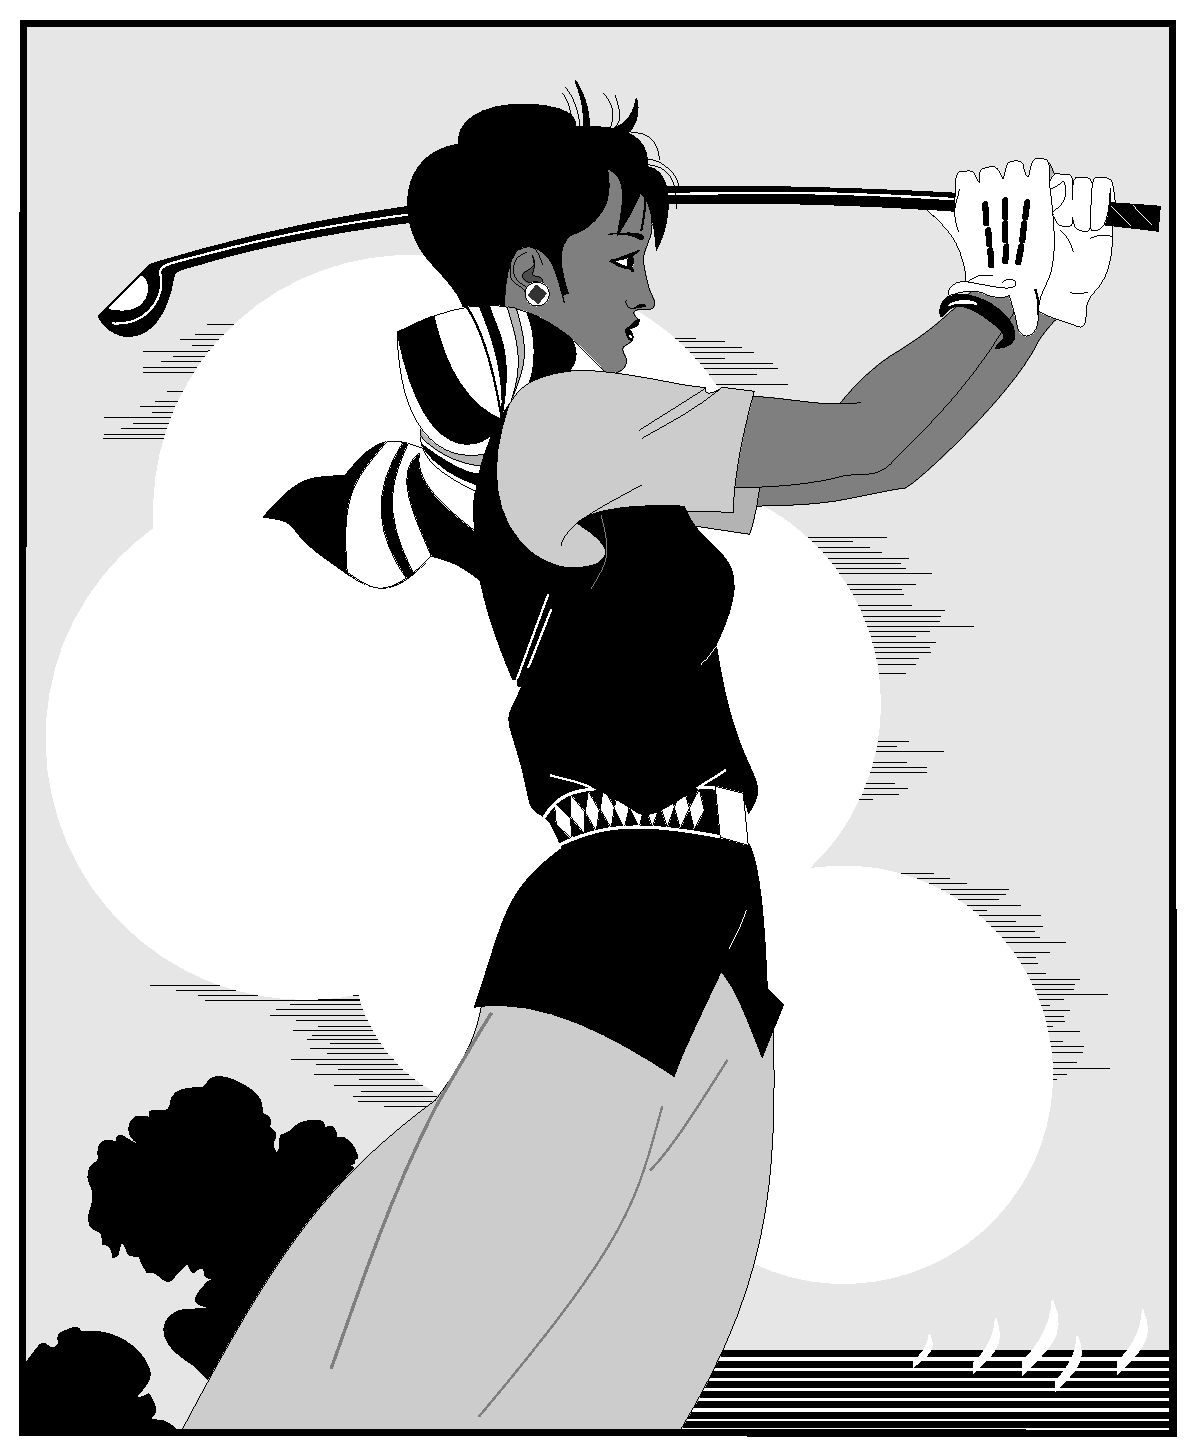
\includegraphics[width = 0.4\textwidth]{golfer}
\bicaption[golfer1]{}{打高尔夫球的人}{Fig.$\!$}{The person playing golf}\vspace{-1em}
\end{figure}

其插入图片的代码及其说明如下。
\vspace{1em}\noindent\hrule
\begin{lstlisting}
\begin{figure}[htbp]
\centering
\includegraphics[width=0.4\textwidth]{文件名(.eps)}
\bicaption[标签名(英文)]{}{中文标题}{Fig.$\!$}
          {English caption (首字母大写)}\vspace{-1em}
\end{figure}
\end{lstlisting}
\noindent\hrule
\begin{lstlisting}
figure环境的可选参数[htbp]表示浮动图形所放置的位置,h (here)表示当前位置,t (top)表示页芯顶部,b (bottom)表示页芯底部,p (page)表示单独一页。在word等软件中,图片通常插入到当前位置,如果当前页的剩余空间不够,图片将被移动到下一页,当前页就会出现很大的空白,其人工调整工作非常不便。由LaTeX提供的浮动图片功能,总是会按h->t->b->p的次序处理选项中的字母,自动调整图片的位置,大大减轻了工作量。
\centering命令将后续内容转换成每行皆居中的格式。
“\includegraphics”的可选参数用来设置图片插入文中的水平宽度,一般表示为正文宽度(\textwidth)的倍数。
\bicaption命令的使用需要调用ccaption宏包,它可以为图片或表格插入双语标题(博士学位论文要求),可选参数“标签名”为英文形式,一般不以图片或表格的数字顺序作为标签,而应包含一定的图片或表格信息,以便于文中引用(若图片、表格、公式、章节和参考文献等在文中出现的先后顺序发生了变化,其标注序号及其文中引用序号也会跟着发生变化,这一点是word等软件所不能做到的)。第4个参数中的“$\!$”表示-1/6个空铅宽度,这样可以缩小Fig.和Table与后面数字序号之间的水平距离。另外,图题或表题并不会因为分页而与图片或表格体分置于两页,章节等各级标题也不会置于某页的最底部,LaTeX系统会自动调整它们在正文中的位置,这也是word等软件所无法匹敌的。
注:硕士学位论文的图表只需要插入中文标题,因此需将\bicaption一句命令替换为如下两条命令(下同):
\caption{中文标题}
\label{标签名(英文)}
\vspace将产生一定高度的竖直空白,必选参数为负值表示将后续文字位置向上提升,参数值可自行调整。em为长度单位,相当于大写字母M的宽度。
引用方法:“见图~\ref{标签名(英文)}”、“如图~\ref{标签名(英文)}~所示”等。
\end{lstlisting}
\noindent\hrule\vspace{1em}
若需要将~2~张及以上的图片并排插入到一行中,则需要采用\verb|minipage|环境,如图~\ref{golfer2}~和图~\ref{golfer3}~所示。
\begin{figure}[htbp]
\centering
\begin{minipage}{0.4\textwidth}
\centering
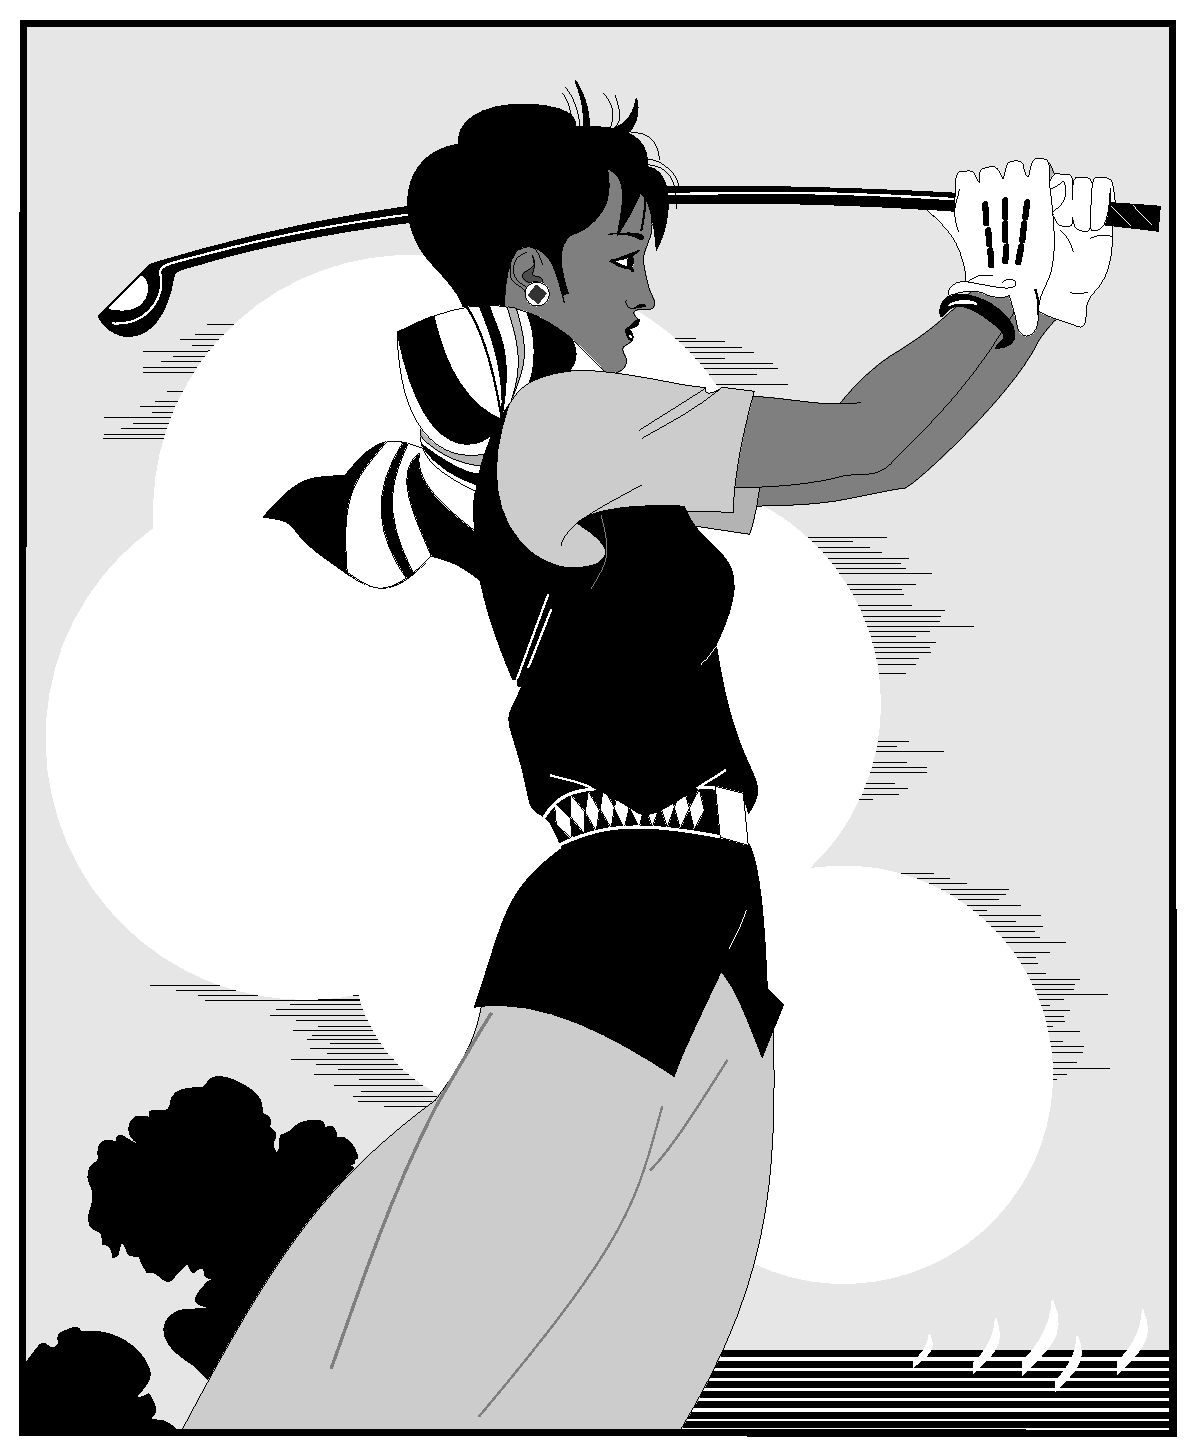
\includegraphics[width=\textwidth]{golfer}
\bicaption[golfer2]{}{打高尔夫球的人}{Fig.$\!$}{The person playing golf}
\end{minipage}
\begin{minipage}{0.4\textwidth}
\centering
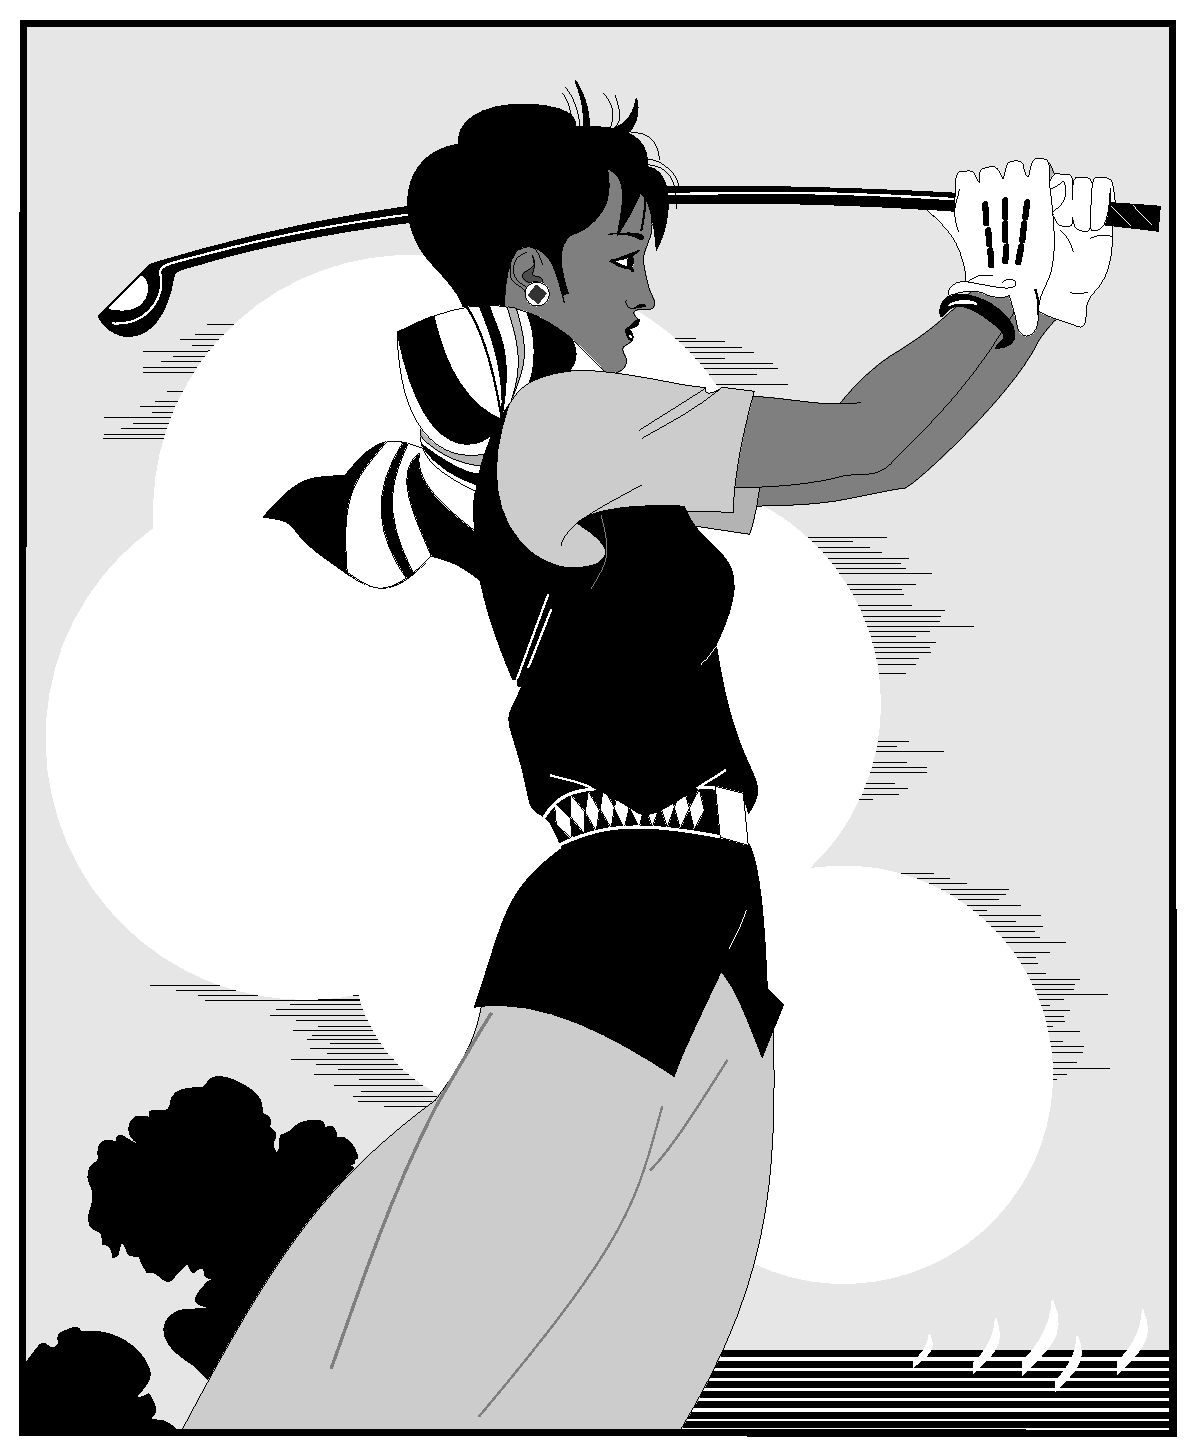
\includegraphics[width=\textwidth]{golfer}
\bicaption[golfer3]{}{打高尔夫球的人}{Fig.$\!$}{The person playing golf}
\end{minipage}\vspace{-1em}
\end{figure}

其代码如下所示。
\vspace{1em}\noindent\hrule
\begin{lstlisting}
\begin{figure}[htbp]
\centering
\begin{minipage}{0.4\textwidth}
\centering
\includegraphics[width=\textwidth]{文件名}
\bicaption[标签名]{}{中文标题}{Fig.$\!$}
          {English caption}
\end{minipage}
\begin{minipage}{0.4\textwidth}
\centering
\includegraphics[width=\textwidth]{文件名}
\bicaption[标签名]{}{中文标题}{Fig.$\!$}
          {English caption}
\end{minipage}\vspace{-1em}
\end{figure}
\end{lstlisting}
\noindent\hrule
\begin{lstlisting}
minipage环境的必选参数用来设置小页的宽度,若需要在一行中插入n个等宽图片,则每个小页的宽度应略小于(1/n)\textwidth。
\end{lstlisting}
\noindent\hrule

\BiSection{具有子图的图片插入方法}{The method of inserting figures with subfigures}

图中若含有子图时,需要调用~subfigure~宏包。博士学位论文规范要求不止总图的标题为中英文形式,其各个子图也应具有中英文形式的标题。
然而~ccaption~宏包却无法实现子图的中英文标题功能,这里采用对\verb|\subfigure|命令进行嵌套的方法来实现子图的中英文标题功能,如图~\ref{golfer4}~所示。

\begin{figure}[htbp]
\centering
\subfigure{\label{golfer41}}\addtocounter{subfigure}{-2}
\subfigure[The person playing golf]{\subfigure[打高尔夫球的人~1]{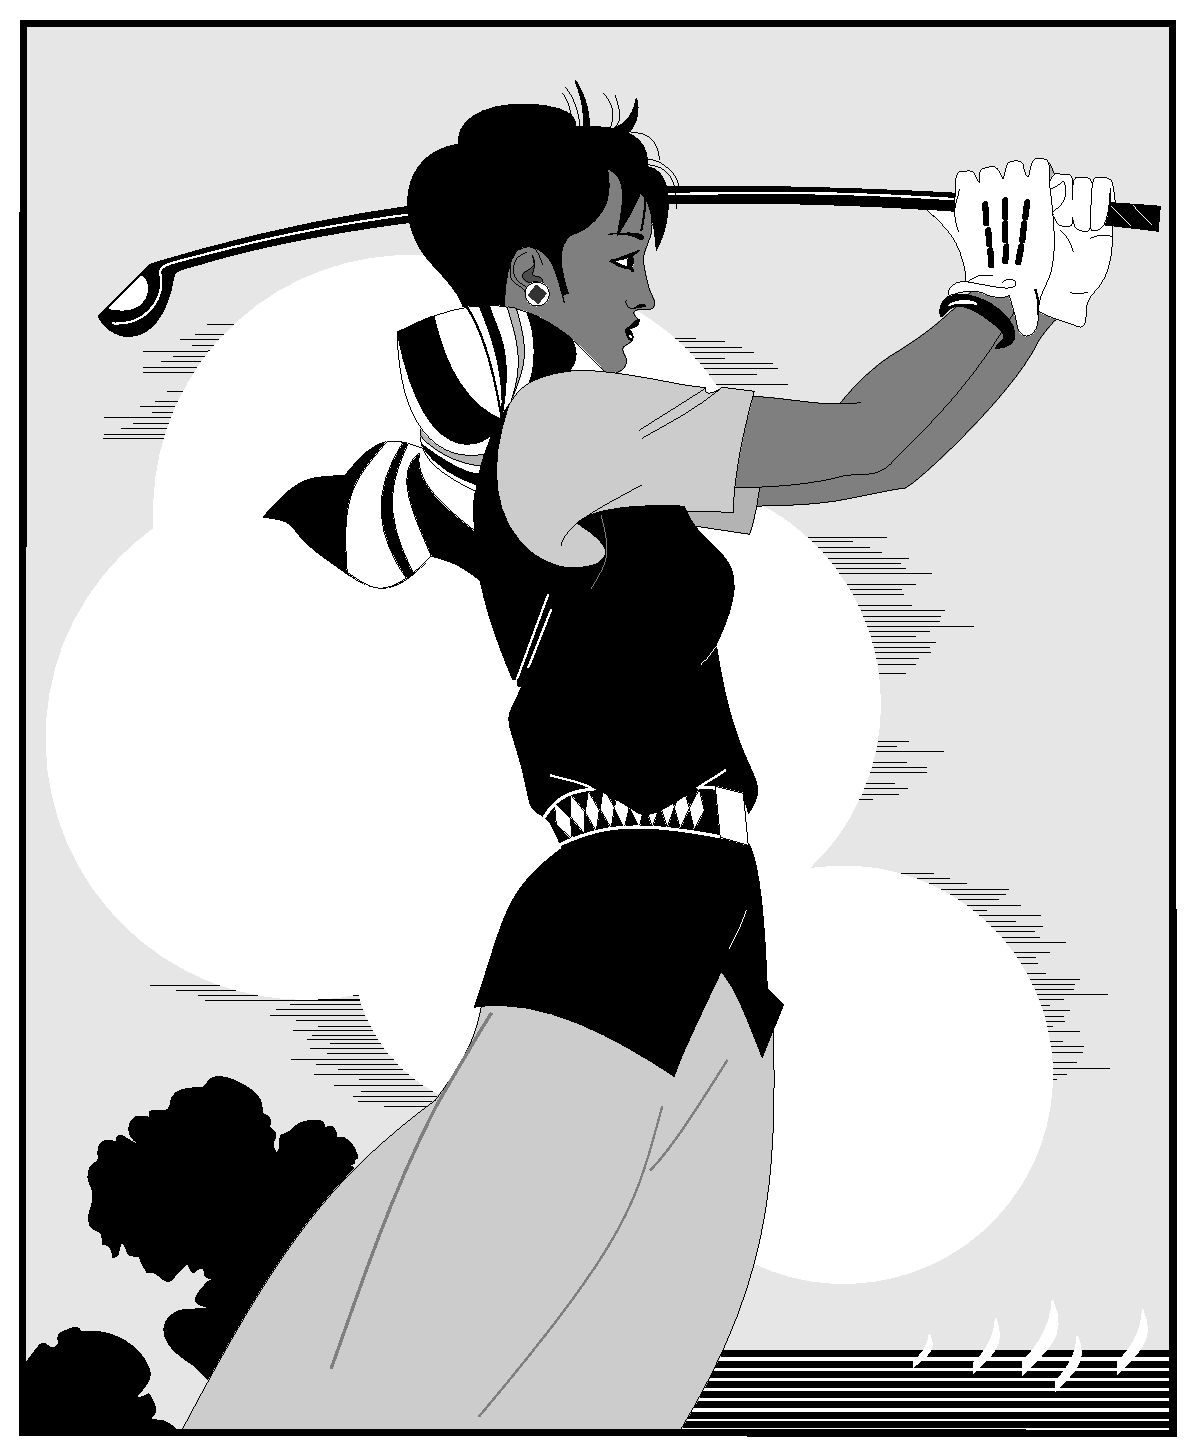
\includegraphics[width=0.4\textwidth]{golfer}}}
\subfigure{\label{golfer42}}\addtocounter{subfigure}{-2}
\subfigure[The person playing golf]{\subfigure[打高尔夫球的人~2]{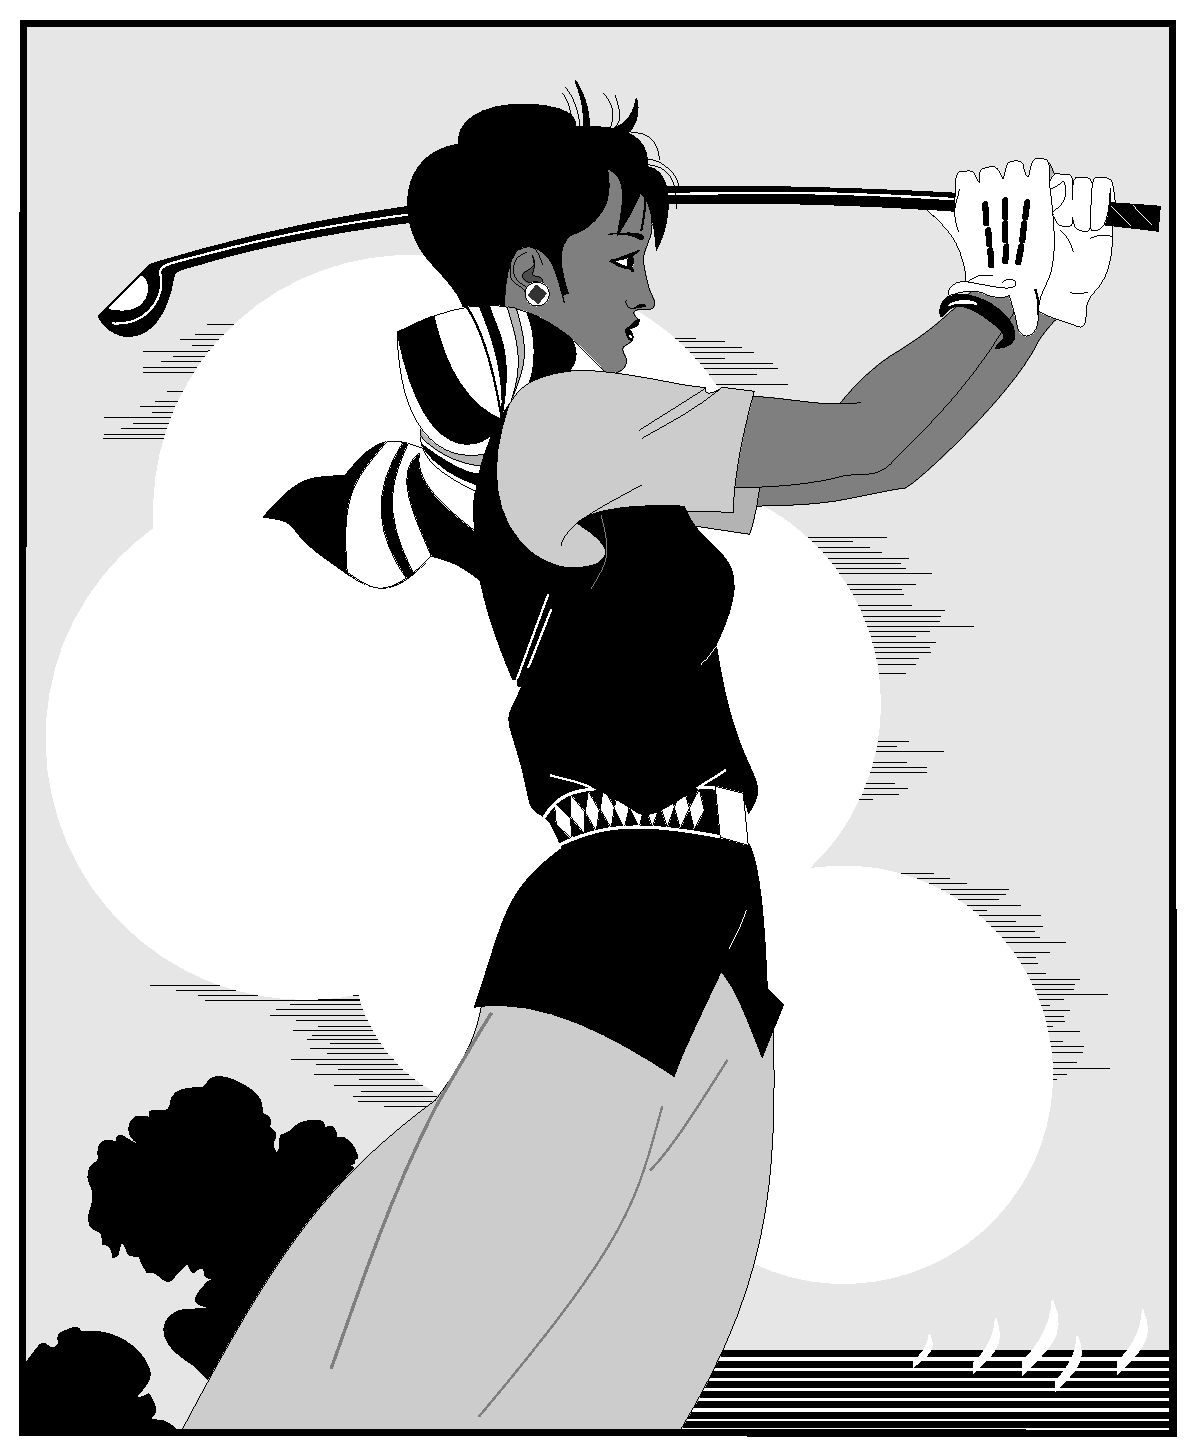
\includegraphics[width=0.4\textwidth]{golfer}}}
\bicaption[golfer4]{}{打高尔夫球的人}{Fig.$\!$}{The person playing golf}\vspace{-1em}
\end{figure}

其代码及其说明如下。
\vspace{1em}\noindent\hrule
\begin{lstlisting}
\begin{figure}[htbp]
\centering
\subfigure{\label{第1个子图标签名}}\addtocounter{subfigure}{-2}
\subfigure[The 1st subfigure caption]{\subfigure[第1个子图标题]
          {\includegraphics[width=0.4\textwidth]{文件名}}}
\subfigure{\label{第2个子图标签名}}\addtocounter{subfigure}{-2}
\subfigure[The 2nd subfigure caption]{\subfigure[第2个子图标题]
          {\includegraphics[width=0.4\textwidth]{文件名}}}
\bicaption[总标签名]{}{中文总标题}{Fig.$\!$}{The total caption}
\vspace{-1em}
\end{figure}
\end{lstlisting}
\noindent\hrule
\begin{lstlisting}
\addtocounter把指定的值加到计数器上,这里是对subfigure计数器进行减2操作。这是因为每插入1个子图,就调用3次\subfigure命令,第1次调用\subfigure命令用来生成紧随其后所插入子图的标签,而之后的双层嵌套调用\subfigure命令用来插入子图并生成该子图的中英文标题。因此,每插入1张子图,subfigure计数器的值就自动加3,为了使得子图的序号能每次加1,则需在每插入1张子图前手动把subfigure计数器的值减2。
\subfigure命令的双层嵌套使用可用来生成中英文标题,其内层\subfigure命令用来插入子图并生成中文标题,外层\subfigure命令将插入的子图和中文标题作为一个整体,生成这个整体的英文标题,因此英文标题会置于中文标题的下面。
硕士学位论文只需要中文标题,其代码如下:
\begin{figure}[htbp]
\centering
\subfigure[第1个子图标题\label{第1个子图标签名}]
          {\includegraphics[width=0.4\textwidth]{文件名}}
\subfigure[第2个子图标题\label{第2个子图标签名}]
          {\includegraphics[width=0.4\textwidth]{文件名}}
\caption{中文总标题}\label{总标签名}
\vspace{-1em}
\end{figure}
引用方法:总图的引用方法同本章第1节,子图的引用方法用\ref{第n个子图标签名}来代替。
\end{lstlisting}
\noindent\hrule\vspace{1em}

子图的引用示例:如图~\ref{golfer41}~和图~\ref{golfer42}~所示。

若想获得插图方法的更多信息,请参见网络上的~\href{ftp://ftp.tex.ac.uk/tex-archive/info/epslatex.pdf}{Using Imported Graphics in \LaTeX and pdf\LaTeX}~文档。 
